\documentclass[11pt]{article}
\usepackage{graphicx}
\usepackage{listings}
\usepackage[utf8]{inputenc}
%Gummi|065|=)
\title{\textbf{Tarea No 2 Algoritmos Genéticos }}
\author{Juan Carlos Olivier Jasso}
\date{Mayo 17, 2016}
\begin{document}

\maketitle



\section {introduccion}


Los Algoritmos Genéticos (AGs) son métodos adaptativos que pueden usarse para resolver problemas de búsqueda y optimización. Están basados en el proceso genético de los organismos vivos. A lo largo de las generaciones, las poblaciones evolucionan en la naturaleza de acorde con los principios de la selección natural y la supervivencia de los más fuertes, postulados por Darwin (1859).\\

Por imitación de este proceso, los Algoritmos Genéticos son capaces de ir creando soluciones para
problemas del mundo real. La evolución de dichas soluciones hacia valores óptimos del problema depende en buena medida de una adecuada codificación de las mismas.  Los principios básicos de los Algoritmos Genéticos fueron establecidos por Holland (1975), y se encuentran bien descritos en varios textos Goldberg (1989), Davis (1991), Michalewicz (1992), Reeves (1993). \\

\newpage
\section{funcionamiento}

En la naturaleza los individuos de una población compiten entre sí en la búsqueda de recursos tales como comida, agua y refugio. Incluso los miembros de una misma especie compiten a menudo en la búsqueda de un compañero. Aquellos individuos que tienen más éxito en sobrevivir y en atraer compañeros tienen mayor probabilidad de generar un gran número de descendientes. Por el contrario, individuos poco dotados producirán un menor número de descendientes. Esto significa que los genes de los individuos mejor adaptados se propagarán en sucesivas generaciones hacia un número de individuos creciente. La combinación de buenas características provenientes de diferentes ancestros, puede a veces producir descendientes súper individuos", cuya adaptación es mucho mayor que la de cualquiera de sus ancestros. De esta manera, las especies evolucionan logrando unas características cada vez mejor adaptadas al entorno en el que viven.\\

Los Algoritmos Genéticos usan una analogía directa con el comportamiento natural. Trabajan con una población de individuos, cada uno de los cuales representa una solución factible a un problema dado. A cada individuo se le asigna un valor o puntuación, relacionado con la bondad de dicha solución. En la naturaleza esto equivaldrá al grado de efectividad de un organismo para competir por unos determinados recursos. Cuanto mayor sea la adaptación de un individuo al problema, mayor será la probabilidad de que el mismo sea seleccionado para reproducirse, cruzando su material genético con otro individuo seleccionado de igual forma. Este cruce producirá nuevos individuos descendientes de los anteriores de los cuales comparten algunas de las características de sus padres.\\

Cuanto menor sea la adaptación de un individuo, menor será la probabilidad de que dicho individuo sea seleccionado para la reproducción, y por tanto de que su material genético se propague en sucesivas generaciones. De esta manera se produce una nueva población de posibles soluciones, la cual reemplaza a la anterior y verídica la interesante propiedad de que contiene una mayor proporción de buenas características en comparación con la población anterior. Así a lo largo de las generaciones las buenas características se propagan a través de la población. Favoreciendo el cruce de los individuos mejor adaptados, van siendo exploradas las áreas más prometedoras del espacio de búsqueda. Si el Algoritmo Genético ha sido bien diseñado, la población convergerá hacia una solución óptima del problema. El poder de los Algoritmos Genéticos proviene del hecho de que se trata de una técnica robusta, y pueden tratar con éxito una gran variedad de problemas provenientes de diferentes áreas, incluyendo aquellos en los que otros métodos encuentran dificultades.\\

\begin{figure}[htp]
\centering
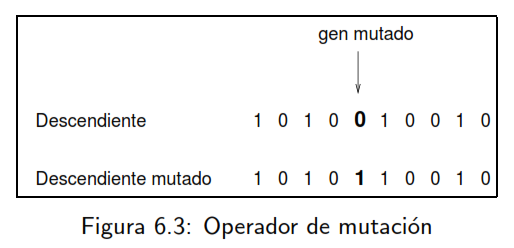
\includegraphics[width=9.5cm]{1.jpg}
\end{figure}

Si bien no se garantiza que el Algoritmo Genético encuentre la solución optima del problema, existe evidencia empírica de que se encuentran soluciones de un nivel aceptable, en un tiempo competitivo con el resto de algoritmos de optimización combinatoria. En el caso de que existan técnicas especializadas para resolver un determinado problema, lo más probable es que superen al Algoritmo Genético, tanto en rapidez como en eficacia. El gran campo de aplicación de los Algoritmos Genéticos se relaciona con aquellos problemas para los cuales no existen técnicas especializadas. Incluso en el caso en que dichas técnicas existan, y funcionen bien, pueden efectuarse mejoras de las mismas hibridándolas con los Algoritmos Genéticos.\\

El Algoritmo Genético Simple

 \begin{verbatim}
BEGIN /* Algoritmo Genético Simple */
Generar una población inicial.
Computar la función de evaluación de cada individuo.
WHILE NOT Terminado DO
BEGIN /* Producir nueva generación */
FOR tamaño población/2 DO

BEGIN /*Ciclo Reproductivo */
Seleccionar dos individuos de la anterior generación,
para el cruce (probabilidad de selección proporcional
a la función de evaluación del individuo).
Cruzar con cierta probabilidad los dos
individuos obteniendo dos descendientes.
Mutar los dos descendientes con cierta probabilidad.
Computar la función de evaluación de los dos
descendientes mutados.
Insertar los dos descendientes mutados en la nueva generación.
END
IF la población ha convergido THEN
Terminado: = TRUE
END
END
\end{verbatim}

\newpage
\section {Explicación}

El Algoritmo Genético Simple, también denominado Canónico, se representa en la figura

Como se verá a continuación, se necesita una codificación o representación del problema, que resulte adecuada al mismo. Además, se requiere una función de ajuste o adaptación al problema, la cual asigna un número real a cada posible solución codificada. Durante la ejecución del algoritmo, los padres deben ser seleccionados para la reproducción, a continuación, dichos padres seleccionados se cruzarán generando dos hijos, sobre cada uno de los cuales actuara un operador de mutación. El resultado de la combinación de las anteriores funciones será un conjunto de individuos (posibles soluciones al problema), los cuales en la evolución del Algoritmo Genético formaran parte de la siguiente población.

\begin{figure}[htp]
\centering
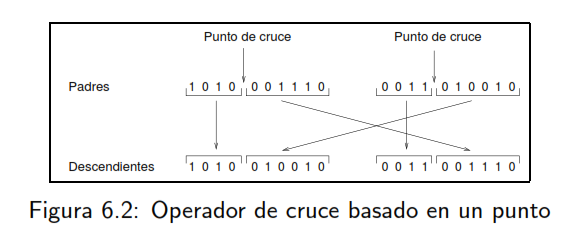
\includegraphics[width=9.5cm]{2.jpg}
\end{figure}


\newpage
\section{Genetic Code}


 \begin{verbatim}
 #include <iostream>
#include <cstdlib>
#include <ctime>    
// for srand, rand
#include <cmath>  // for cos, sin, pow
using namespace std;

// función de evalucion donde el máximo será encontrado
double f(double x){
 return cos(x) - sin(2*x); // Se devuelve como resultado la expresión evaluada
}

//función de evaluación de vlaor individual
double f_value(double (*func)(double), int* arr, int& N, double a,double b)
{
 double res;
 double m = 0.0;
 for(int j=0;j<N;j++)
 {
  double k = j;
  m+= arr[N-j-1]*pow(2.0,k);
 }
 double x = a + m*(b-a)/(pow(2.0,N)-1.0);
 res = func(x);
 return res;
}

// x_value en maximo global
double x_value(int* arr, int& N,double a,double b)
{
 double m = 0.0;
 for(int j=0;j<N;j++)
 {
  double k = j;
  m += arr[N-j-1]*pow(2.0,k);
 }
 double x = a + m*(b-a)/(pow(2.0,N)-1.0);
 return x;
}

// Establce de manera aleatoria la población dentro de la granja
void setup(int** farm,int M, int N)
{
 srand((unsigned long) time(NULL));
 for(int j=0;j<M;j++)
  for(int k=0;k<N; k++)
   farm[j][k] = rand()%2;
}

// Cruza dos individuos
void crossings(int** farm, int& M, int& N, double &a, double& b)
{
 int K = 2;
 int** temp = new int* [K];
 for(int i=0;i<K;i++)
  temp[i] = new int[N];

 double res[4];
 int r1 = rand()%M;
 int r2 = rand()%M;
 // Este random devuelve un valor entre 0 y 1 menor que este parametro
 while(r2 == r1)
  r2 = rand()%M;
 res[0] = f_value(f, farm[r1], N, a, b);
 res[1] = f_value(f, farm[r2], N, a, b);

//Se guaradn em una arreglo temporal los valores
for(int j=0;j<N;j++)
{
 temp[0][j] = farm[r1] [j] ;
 temp[1][j] = farm[r2] [j] ;
}
int r3 = rand()%(N-2) + 1;
 for(int j=r3;j<N;j++)
 {
  temp[0][j] = farm[r2][j];
  temp[1][j] = farm[r1][j] ;
 }
  res[2] = f_value(f ,temp[0] ,N,a,b);
  res[3] = f_value(f ,temp[1] ,N,a,b);
  if(res[2] > res[0])
  {
   for(int j=0;j<N;j++)
    farm[r1] [j] = temp[0] [j] ;
    res[0] = res [2] ;
  }

  if(res[3] >res[1])
  {
   for(int j=0;j<N;j++)
    farm[r2][j] = temp[1] [j] ;
   res[1] =res[3];
  }

  for(int j=0;j<K;j++)
   delete[] temp[j] ;
   delete[] temp;
}

// Funcion en la cual ocurre una mutuación, para un individuo

void mutate(int** farm, int& M, int& N, double& a,double& b)
{
  double res[2];
  int r4=rand()%N;
  int r1=rand()%M;
  

res[0] = f_value(f ,farm[r1] ,N,a,b);
  int v1 = farm[r1] [r4];
    
// Revisa que la posición tenga un individuo para entonces realizar la openacion en la grana
  if(v1 == 0) farm[r1][r4] = 1;
  if(v1 == 1) farm[r1][r4] = 0;

//Funcion que devuelve su valor en individual
  double a1 = f_value(f, farm[r1], N,a,b);
  if(a1 < res[0])
   farm[r1][r4] = v1;

  int r5 = rand()%N;
  int r2 = rand()%M;
  res[1] = f_value(f, farm[r2] ,N,a,b);
  int v2 = farm[r2][r5];
  if(v2 == 0) farm[r2][r5] = 1;
  if(v2 == 1) farm[r2][r5] = 0;
  double a2 = f_value(f, farm[r2], N,a,b);
  if(a2 < res[1]) farm[r2][r5] = v2;
}

int main(void)
{
 int M = 12; // Población de la granjas actualmente 12
 int N = 10; // llongitud de estrin binario

 int** farm = new int*[M];      // se reserva la memoria para que el apuntador la pueda usar
 for(int i=0;i<M;i++) { farm[i] = new int[N]; }     //Para cada uno se hace lo mismo malloc


 setup(farm,M,N);               //Creación de la granja
 double a=0.0,b=6.28318;        //Intervalo (a , b)

 for(int k=0;k<1000;k++)
 {
  crossings(farm,M,N,a,b);
  mutate(farm,M,N,a,b);
 } //endforloop

 for (int j=0;j<N;j++)
  cout << "farm[l] [" << j << "] = " << farm[1] [j] << endl;
  cout << endl;

 for(int j=0;j<M;j++)
  cout << "fitness f_value[" << j << "] = "
   << f_value(f ,farm[j] ,N,a,b)
   << " " << "x_value[" << j << "]=" << x_value(farm[j] ,N,a,b) << endl;

// Limpieza de memoria
 for(int j=0;j<M;j++)
  delete[] farm[j];
  delete[] farm;
  return 0;


}







\end{verbatim}



\end{document}
